\documentclass[10pt, compress,urlcolor=blue]{beamer}

\usetheme{CambridgeUS}

\usepackage{fontspec}

\usepackage{hyperref}

\usepackage{booktabs}
\usepackage[english, francais]{babel} 
\usepackage[scale=2]{ccicons}
\usepackage{minted}
\usepackage{amsmath}


\usepackage{tikz}
\usepackage{tikz-qtree}

\usemintedstyle{trac}

\title{Atelier OCR et HTR}
%\date{\today}
%\date{13 mars 2017}

\author{Jean-Baptiste Camps}
\institute{Masters HNC et TNAH | ENC (PSL)}

\setbeamersize{description width=0.47cm}

\makeatletter 

%\AtBeginSection[]{% 
%	\begin{frame}{Plan}%
%	\small
%	\tableofcontents[currentsection]%
%\end{frame} }

\AtBeginSection[]{% 
\begin{frame}{Plan}%
\small
\tableofcontents[currentsection]%
\end{frame} }


\makeatother 

\begin{document}

\maketitle

\begin{frame}{Acquisition du texte}
    
    Dans la constitution d'un corpus de textes, la première phase est bien sûr l'acquisition du contenu des textes envisagés.
\begin{description}
	\item[Transcription] des témoins, selon les critères scientifiques du projet (transcriptions allographétiques, graphématiques, normalisées; édition critique; etc.). Méthode souvent la plus sûre, mais aussi la plus lente;
	\item[``Transcription'' assistée par ordinateur] en utilisant un algorithme permettant la reconnaissance optique de caractères (\textit{optical character recognition} ou \textsc{ocr}) imprimés, ou la reconnaissance des écritures manuscrites (\textit{handwritten text recognition} ou \textsc{htr}).
	\item[Téléchargement] de textes depuis des corpus en lignes, des sites d'édition électronique, des bases de données d'éditeurs, etc.
\end{description}
    
\end{frame}


\begin{frame}{OCR et HTR}
    
    \begin{columns}
	\begin{column}{0.48\textwidth}
		Reconnaissance optique des caractères (imprimés)\\
		\textit{Optical character recognition} (\textsc{ocr})
		\begin{itemize}
		    \item ``problème résolu'' de l'informatique;
		    \item aisé d'obtenir des taux d'erreur caractère (CER) < 2\%;
		    \item outils libres: \texttt{Tesseract} 4, …;
		    \item existence de modèles génériques (par langue).
		\end{itemize}
	\end{column}
	\begin{column}{0.48\textwidth}
		Reconnaissance des écritures manuscrites\\
		\textit{Handwritten text recognition} (\textsc{htr})
		\begin{itemize}
		    \item très peu fonctionnel jusqu'à ces dernières années;
		    \item nouveaux développements: IA (réseaux de neurones récurrents LSTM…);
		    \item outils libres: \texttt{Kraken}, …
		    \item modèles spécifiques à entraîner (pour chaque main, écriture,…);
		    \item on progresse petit à petit sur la généralité des modèles.
		\end{itemize}
	\end{column}
\end{columns}
    
\end{frame}

%Mesure d'erreur: character error rate (CER)
%etc.

%Éléments à reprendre:
% - article Albi
% - projet CNRS


\begin{frame}{Les étapes}
		\begin{enumerate}
			\item traitement des images;
			\item analyse de la mise en page et identification des lignes;
			\item reconnaissance des caractères;
			\item d'éventuels post-traitements, visant à améliorer les résultats.
		\end{enumerate}
	\end{frame}
	
%Les outils: 
% Outils spécifiques aux données patrimoniales
%   - Oriflamms
%   - Transkribus

% Outils généralistes
%   - OCRopy / CLSTM
%   - OCRopy 2
%   - Tesseract 4

\section{Traitement des images}


\begin{frame}{}
    \begin{columns}
	\begin{column}{0.45\textwidth}
		Dans une démarche de reconnaissance des écritures, la qualité des images
		et de leurs traitements est cruciale.
	\end{column}
	\begin{column}{0.45\textwidth}
		Besoins:
		\begin{enumerate}
		    \item images en 300 DPI minimum;
		    \item redressées, débruitées;
		    \item binarisées.
		\end{enumerate}
		Outils: logiciels de traitement d'image, par ex. \texttt{ScanTailor}
	\end{column}
\end{columns}
    
\end{frame}

\begin{frame}{T.P. ScanTailor}
    
    \begin{enumerate}
        \item Démarrer un nouveau projet;
        \item charger les images du dossier \texttt{src} (Mer des Histoires ou Cid à défaut);
        \item suivre les différentes étapes dans le logiciel;
        \item exporter en tiff binarisé 600 DPI.
    \end{enumerate}
    
\end{frame}

\section{Analyse de la mise en page}

\begin{frame}{Analyser la mise en page}
    \begin{columns}
	\begin{column}{0.45\textwidth}
		\textbf{Identifier}
		\begin{itemize}
		    \item zones de texte;
		    \item décoration;
		    \item colonnes;
		    \item lignes;
		    \item mots;
		    \item lettres.
		\end{itemize}
	\end{column}
	\begin{column}{0.45\textwidth}
		\textbf{Approches}
		\begin{itemize}
		    \item Sans apprentissage, par ex.
		    \begin{itemize}
		        \item \texttt{OCRopy} 1;
		        \item \textsc{Oriflamms} (\textsc{IRHT});
		        \item \texttt{Kraken};
		    \end{itemize}
		    \item fondée sur des méthodes d'apprentissage (IA), par ex.
		    \begin{itemize}
		        \item \texttt{OCRopy} 2?
		    \end{itemize}
 		\end{itemize}
	\end{column}
\end{columns}
    
\end{frame}


\begin{frame}[fragile]
\frametitle{Installer Kraken}

\alert{Une installation de python $\geq 3.6$ est nécessaire.}

Sur Ubuntu, il vous faut les paquets \texttt{python3.6},  \texttt{python3.6-dev} et \texttt{pip3}.

% python3.6 -m venv env
\begin{minted}{bash}
# Créer un environnement virtuel (optionnel)
$ virtualenv env -p /usr/bin/python3.6
# l'activer (optionnel)
$ source env/bin/activate
# installer
$ pip3 install kraken
# Utilisation basique
# installer le modèle par défaut
$ kraken get default
# lister les modèles disponibles au téléchargement 
$ kraken list
\end{minted}
    
\end{frame}



\begin{frame}[fragile]
\frametitle{Analyser la mise en page avec \texttt{Kraken}: étape par étape}
    Depuis la racine du dossier:
\begin{block}{\alert{Si les images n'ont pas été prétraitées}}
\begin{minted}{bash}
#Binariser les images (si pas déjà fait avec ScanTailor)
$ kraken -I "src/*" -o .png binarize
# Segmentation en lignes
$ kraken -I "src/*.png" -o .json segment
# OU les deux d'un coup
kraken -I "src/*" -o .json binarize segment
\end{minted}
\end{block}


\begin{block}{\alert{Si elles l'ont été}}
\begin{minted}{bash}
# Segmentation en lignes
$ kraken -I "tif/*" -o .json segment
\end{minted}
\end{block}

\end{frame}


\begin{frame}[fragile]
\frametitle{Tout-en-un}

\begin{block}{Pour binariser, segmenter et générer un fichier de transcription}
\begin{minted}{bash}
# Pour générer un fichier de transcription
$ ketos transcribe -o gt.html tif/*
\end{minted}
\end{block}
    
\end{frame}

\section{OCR et HTR}

\begin{frame}
		\frametitle{Différentes solutions techniques}
		
		%Différents outils de ROC/ROM, et paradigmes techniques
		%Lequel est le plus adapté, choix d'Ocropy/CLSTM
		
		\begin{itemize}
			\item approches segmentées ou non segmentées;
			\item mesures de distance; méthodes statistiques ou d'intelligence artificielle (réseaux de neurones convolutifs ou récurrents, LSTM 1D, LSTM 2D, etc.);
			\item outils directement opérationnels ou nécessitant un entraînement.
		\end{itemize}
		
	%	\pause
		
		\begin{block}{Ocropy, CLSTM et Kraken}
			\href{https://github.com/tmbdev/ocropy}{\texttt{OCRopy}} et \href{http://github.com/tmbdev/clstm}{CLSTM} développés par Thomas M. Breuel; \href{https://github.com/mittagessen/kraken}{\texttt{Kraken}}, \textit{fork} d'\texttt{OCRopy} développé par Ben Kiessling (PSL), \texttt{Calamari} (\textit{fork} de Kraken)…
			\begin{itemize}
				\item approche non segmentées;
				\item réseaux de neurones récurrents (LSTM);
				\item \textit{open source} et nécessitant l'entraînement d'un modèle.
			\end{itemize}
		\end{block}
		
	\end{frame}
	
		
	\begin{frame}[fragile]
		\frametitle{Un apprentissage guidé}
		
		\only<1>{
			
			\centering
			\begin{tikzpicture}
	\node[draw, rectangle, rounded corners=3pt] (P) at (-4,6)
	{Prétraitement des images};%
	\node[draw, rectangle, rounded corners=3pt] (A) at (-3,5)
	{Analyse mise en page};%
	\node[draw, rectangle, rounded corners=3pt] (GT) at (0,2.7)
	{Vérité de terrain};
	\node[draw, rectangle, rounded corners=3pt] (T) at (4,2.7)
	{Entraînement};
	\node[draw, rectangle, rounded corners=3pt] (TT) at (2,0.5)
	{Test};
	\node[draw, rectangle, rounded corners=3pt] (O) at (2,-0.5)
	{Sortie};
	
	\draw[->,>=latex] (P) -- (A) ;
	\draw[->,>=latex] (A) -- (GT) node[midway,sloped,above] {transcription}; 
	\draw[->,>=latex] (GT) -- (T) ; 
	\draw[->,>=latex] (T) -- (TT) ;
	\draw[->,>=latex] (TT) -- (GT) node[midway,sloped,above] {relecture};
	\draw[->,>=latex] (TT) -- (O) ;
	\end{tikzpicture}
			
		} 
		
		
	\only<2>{
			\begin{block}{Entraînement sur un ms. (ici Roland d'Oxford)}\centering
				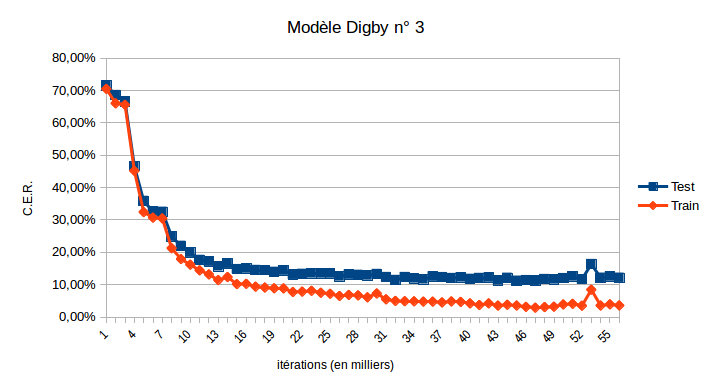
\includegraphics[width=\textwidth]{img/entrainementDigby3.png}
				
			\end{block}
		}
		
		\only<3>{
			\begin{block}{Résultats}
				\begin{itemize}
					\item pour un imprimé ancien, des taux d'erreur de l'ordre de 1\% sont atteignables…
					\item pour un ms., des taux inférieurs à 10\% sont atteignables rapidement, $>$5\% plus difficiles;
					\item cas du Digby 23, env. 400 lignes d'entraînement,
					taux de succès de 89,16\% en test, et 93\% sur l'ensemble des données;
				\end{itemize}
			\end{block}
			\begin{block}{Pour un modèle un peu plus général}
				\href{https://github.com/Jean-Baptiste-Camps/FROC-MSS}{https://github.com/Jean-Baptiste-Camps/FROC-MSS}
				\begin{itemize}
					\item 4 manuscrits différents du XII\ieme{}-XIII\ieme{};
					\item 3000 lignes env.
					\item CER de 8\% en test (7\% en ignorant l'espacement).
				\end{itemize}
			\end{block}
			
		}
	
		
	\end{frame}

\begin{frame}[fragile]
\frametitle{Évaluation et confusions fréquentes}

\begin{minted}{bash}
Evaluating model_froc.mlmodel
Evaluating 100 %
=== report  ===

13645   Characters
1107    Errors
91.89 %  Accuracy

585     Insertions
156     Deletions
366     Substitutions

Errors  Correct-Generated
91      { SPACE } - {  }
67      { ı } - {  }
56      {  } - { SPACE }
36      { COMBINING ACUTE ACCENT } - {  }
32      { n } - {  }
\end{minted}
    
\end{frame}
	
%# N.B.: les commandes peuvent se combiner. 
%# Tout-en-un avec le modèle par défaut
%$ kraken -i src/50rb.jpg texte.txt binarize segment ocr

\subsection{Préparation des données}

\begin{frame}[fragile]
\frametitle{T.P. \texttt{Kraken}: Préparation des données}

\textbf{1. Essayer d'appliquer un modèle déjà entraîné}
\begin{minted}[breaklines]{bash}
# Lancer la reconnaissance 
# et extraire un fichier de correction
$ ketos transcribe -o gt.html --prefill model_best.mlmodel tif/*.tif
# Ou, si ça vous satisfait, extraire directement un fichier texte
$ kraken -I "tif/*.tif" -o .txt segment ocr -m model_best.mlmodel
# ou hocr
$ kraken -I "tif/*.tif" -o .txt segment ocr -m model_best.mlmodel
\end{minted}

Pas terrible… Mais comment améliorer le modèle?

\textbf{2. Corriger / transcrire}
\end{frame}

\subsection{Entraîner}

\begin{frame}[fragile]
\frametitle{T.P. \texttt{Kraken}: préparer l'entraînement}


\textbf{3. Extraire et entraîner}
\begin{minted}[breaklines]{bash}
#Extraire et normaliser les caractères
$ ketos extract --output book --normalization NFD gt.html
\end{minted}

Ensuite idéalement, 80\% des données vont servir à entraîner, 10\% à évaluer les modèles pendant l'entraînement, 10\% à tester le modèle retenu (on peut faire 90\% - 10\% si la précision de l'évaluation n'est pas critique).

\begin{itemize}
    \item \alert{il est recommandé de faire cette répartition de manière aléatoire};
    \item \alert{il est possible d'accroître artificiellement le nombre de lignes d'entraînement, en bruitant de différentes manières les lignes de GT.}
\end{itemize}
\end{frame}

\begin{frame}[fragile]
\frametitle{Création des jeux \texttt{train}, \texttt{val} et \texttt{test}}
	
\begin{block}{Sélection des pages à transcrire}
	Lorsque vous préparez des données d'entraînement, il peut être préférable de ne pas transcrire des pages immédiatement contiguës, mais de les sélectionner aléatoirement dans l'ensemble du document.

	$\rightarrow$ éviter des biais dus à des changements de fonte, mise en page, etc.
\end{block}	

\begin{block}{Répartition en \texttt{train} / \texttt{val} / \texttt{test}}
	Pour des raisons similaires, et \alert{surtout pour des documents anciens} ou irréguliers, il vaut mieux
	sélectionner aléatoirement des lignes de chaque page pour les séparer en \texttt{train} / \texttt{val} / \texttt{test}.
	
\end{block}	

On peut créer un script Python ou autre pour ce faire:
\begin{minted}{bash}
$ python3 ../randomise_data.py book/*.png
\end{minted}
	
\end{frame}


\begin{frame}[fragile]
\frametitle{Apparté: augmentation artificielle des données d'entraînement}

\textbf{Constat}: \alert{transcrire coûte cher} (temps, effort, …). 

Pour obtenir augmenter les données d'entraînement avec moins d'effort, on peut:

\begin{itemize}
	\item générer des lignes arbitraires de textes, si l'on dispose de la fonte (commande \texttt{ketos linegen} dans Kraken);
	\item appliquer diverses déformations et bruiter les lignes (pseudo-tâches, trous, bavures, courbures, etc.)
\end{itemize}

Un bon outil: \texttt{Doccreator}, \href{http://doc-creator.labri.fr}{http://doc-creator.labri.fr}, qui permet de:
\begin{itemize}
	\item extraire une pseudo-fonte à partir de documents;
	\item multiplier les lignes par autant de déformations 2D ou 3D que l'on souhaite.
\end{itemize}

Permet en général des gains modestes (1 ou 2\% de CER), mais appréciables.

\end{frame}

\begin{frame}[fragile]
\frametitle{T.P. \texttt{Kraken}: lancer l'entraînement}
    
On peut ensuite lancer un entraînement (de zéro ou à partir du modèle précédent, aux choix). 
\begin{minted}{bash}
#Lancer l'entraînement
$ ketos train -t train.txt -e val.txt
\end{minted}

N.B: de nombreux autres paramètres sont disponibles, liés au modèle et à l'entraînement.

Si les données n'ont pas été normalisées auparavant, on peut utiliser l'option
`-u NFD` (normalisation Unicode).

\end{frame}

\subsection{Évaluer les résultats}

\begin{frame}[fragile]
\frametitle{T.P. \texttt{Kraken}: Test des résultats}


\textbf{4. Tester les résultats}

Une fois que l'entraînement a atteint un niveau satisfaisant, ou quand les paramètres de l'\textit{early stopping} ont mené à l'interrompre (l'erreur a cessé de décroître suffisamment pendant un nombre donné d'époques)
on peut tester la qualité du résultat, 

\begin{minted}{bash}
# Test du meilleur modèle et confusions de caractères
$ ketos test -m model_best.mlmodel -e test.txt
\end{minted}

%# Test des erreurs de différents modèles, comparativement
%for i in *.mlmodel; do 
%    echo "$i" >> modeltest 
%    $ ketos test -m model_best.mlmodel book2/*/*.png>>modeltest 
%done

\end{frame}

\section{Et après?}

\begin{frame}{Post-correction}
	Une fois que l'on a un modèle aux résultats satisfaisants, on peut l'appliquer à l'ensemble du document. Mais, quel que soit sa précision, il risque de rester tout de même des erreurs.
	
	Il est délicat d'échapper à une relecture de l'ensemble, dans la plupart des cas, mais certains outils permettent d'accélérer ce processus:
	
	\begin{itemize}
		\item outils type `correcteurs orthographiques' pour les langues modernes / standardisées;
		\item modèles linguistiques un peu plus complexes pour les états anciens de langue.
	\end{itemize}
	
Un exemple: \texttt{PoCoTo} (\href{https://github.com/cisocrgroup/PoCoTo}{https://github.com/cisocrgroup/PoCoTo}).
	
\end{frame}



\end{document}

%\begin{columns}
%	\begin{column}{0.45\textwidth}
%		contenu...
%	\end{column}
%	\begin{column}{0.45\textwidth}
%		contenu...
%	\end{column}
%\end{columns}